% Options for packages loaded elsewhere
\PassOptionsToPackage{unicode}{hyperref}
\PassOptionsToPackage{hyphens}{url}
%
\documentclass[
]{article}
\usepackage{amsmath,amssymb}
\usepackage{lmodern}
\usepackage{iftex}
\ifPDFTeX
  \usepackage[T1]{fontenc}
  \usepackage[utf8]{inputenc}
  \usepackage{textcomp} % provide euro and other symbols
\else % if luatex or xetex
  \usepackage{unicode-math}
  \defaultfontfeatures{Scale=MatchLowercase}
  \defaultfontfeatures[\rmfamily]{Ligatures=TeX,Scale=1}
\fi
% Use upquote if available, for straight quotes in verbatim environments
\IfFileExists{upquote.sty}{\usepackage{upquote}}{}
\IfFileExists{microtype.sty}{% use microtype if available
  \usepackage[]{microtype}
  \UseMicrotypeSet[protrusion]{basicmath} % disable protrusion for tt fonts
}{}
\makeatletter
\@ifundefined{KOMAClassName}{% if non-KOMA class
  \IfFileExists{parskip.sty}{%
    \usepackage{parskip}
  }{% else
    \setlength{\parindent}{0pt}
    \setlength{\parskip}{6pt plus 2pt minus 1pt}}
}{% if KOMA class
  \KOMAoptions{parskip=half}}
\makeatother
\usepackage{xcolor}
\usepackage[margin=1in]{geometry}
\usepackage{graphicx}
\makeatletter
\def\maxwidth{\ifdim\Gin@nat@width>\linewidth\linewidth\else\Gin@nat@width\fi}
\def\maxheight{\ifdim\Gin@nat@height>\textheight\textheight\else\Gin@nat@height\fi}
\makeatother
% Scale images if necessary, so that they will not overflow the page
% margins by default, and it is still possible to overwrite the defaults
% using explicit options in \includegraphics[width, height, ...]{}
\setkeys{Gin}{width=\maxwidth,height=\maxheight,keepaspectratio}
% Set default figure placement to htbp
\makeatletter
\def\fps@figure{htbp}
\makeatother
\setlength{\emergencystretch}{3em} % prevent overfull lines
\providecommand{\tightlist}{%
  \setlength{\itemsep}{0pt}\setlength{\parskip}{0pt}}
\setcounter{secnumdepth}{5}
\newlength{\cslhangindent}
\setlength{\cslhangindent}{1.5em}
\newlength{\csllabelwidth}
\setlength{\csllabelwidth}{3em}
\newlength{\cslentryspacingunit} % times entry-spacing
\setlength{\cslentryspacingunit}{\parskip}
\newenvironment{CSLReferences}[2] % #1 hanging-ident, #2 entry spacing
 {% don't indent paragraphs
  \setlength{\parindent}{0pt}
  % turn on hanging indent if param 1 is 1
  \ifodd #1
  \let\oldpar\par
  \def\par{\hangindent=\cslhangindent\oldpar}
  \fi
  % set entry spacing
  \setlength{\parskip}{#2\cslentryspacingunit}
 }%
 {}
\usepackage{calc}
\newcommand{\CSLBlock}[1]{#1\hfill\break}
\newcommand{\CSLLeftMargin}[1]{\parbox[t]{\csllabelwidth}{#1}}
\newcommand{\CSLRightInline}[1]{\parbox[t]{\linewidth - \csllabelwidth}{#1}\break}
\newcommand{\CSLIndent}[1]{\hspace{\cslhangindent}#1}
\usepackage{titling}
\pretitle{\begin{center} 
\includegraphics[width=2in,height=2in]{logo.jpg}\LARGE\\}
\posttitle{\end{center}}
\usepackage{listings}
\usepackage{xcolor}
\definecolor{customgreen}{rgb}{0,0.6,0}
\definecolor{customgray}{rgb}{0.5,0.5,0.5}
\definecolor{custommauve}{rgb}{0.6,0,0.8}
\lstset{ basicstyle=\small, breaklines=true, commentstyle=\color{customgreen}, firstnumber=1, frame=single, keepspaces=true, keywordstyle=\color{blue}, numbers=left, numbersep=10pt, numberstyle=\tiny\color{customgray}, rulecolor=\color{black}, showspaces=false, showstringspaces=false, showtabs=false, stepnumber=1, stringstyle=\color{custommauve}, tabsize=2, }
\ifLuaTeX
  \usepackage{selnolig}  % disable illegal ligatures
\fi
\IfFileExists{bookmark.sty}{\usepackage{bookmark}}{\usepackage{hyperref}}
\IfFileExists{xurl.sty}{\usepackage{xurl}}{} % add URL line breaks if available
\urlstyle{same} % disable monospaced font for URLs
\hypersetup{
  pdftitle={AWS Machine Learning Engineer Nanodegree},
  pdfauthor={Masinde Mtesigwa Masinde},
  hidelinks,
  pdfcreator={LaTeX via pandoc}}

\title{AWS Machine Learning Engineer Nanodegree}
\author{Masinde Mtesigwa Masinde}
\date{2023-03-10}

\begin{document}
\maketitle

{
\setcounter{tocdepth}{3}
\tableofcontents
}
\newpage

\hypertarget{definition}{%
\section{Definition}\label{definition}}

\hypertarget{project-overview}{%
\subsection{Project Overview}\label{project-overview}}

Electronic Health records or Electronic Medical Records data is the data
being collected when we see a doctor, pick up a prescription at the
pharmacy, or even from a visit to the dentist.

This data is used for a variety of use-cases. From personalizing
healthcare to discovering novel drugs and treatments to helping
providers diagnose patients better and reduce medical errors.

Diabetes mellitus, or simply diabetes, is a leading non-communicable
disease (NCD) globally, almost doubling in cases since 1980. It is a
chronic illness that develops either when the pancreas are not able to
generate sufficient insulin or when the body does not utilize the
insulin produced effectively. There is no cure for this disease.
Diabetes is thought to result from a combination of genetic and
environmental factors. Several risk factors that are attributed to
diabetes include ethnicity, family history of diabetes, age, excess
weight, unhealthy diet, physical inactivity, and smoking. In addition to
this, the absence of early detection of diabetes has been known to
contribute to the development of other chronic diseases such as kidney
disease.

\hypertarget{dataset}{%
\subsection{Dataset}\label{dataset}}

This dataset is originally from the National Institute of Diabetes and
Digestive and Kidney Diseases. The objective of the dataset is to
diagnostically predict whether or not a patient has diabetes, based on
certain diagnostic measurements included in the dataset. Several
constraints were placed on the selection of these instances from a
larger database. In particular, all patients here are females at least
21 years old of Pima Indian heritage.

The datasets consists of several medical predictor variables and one
target variable, Outcome. Predictor variables includes the number of
pregnancies the patient has had, their BMI, insulin level, age, and so
on\textsuperscript{\protect\hyperlink{ref-ehr}{1}}.

\hypertarget{problem-statement}{%
\subsection{Problem Statement}\label{problem-statement}}

Diabetes mellitus, or simply diabetes, is a leading non-communicable
disease (NCD) globally, almost doubling in cases since 1980. It is a
chronic illness that develops either when the pancreas are not able to
generate sufficient insulin or when the body does not utilize the
insulin produced effectively

Can you build a machine learning model to accurately predict whether or
not the patients in the dataset have diabetes or not?

This problem is a classification problem. In this problem, a classifier
is built that can be trained using the given dataset and can be used to
predict diabetes class from a given input dataset. The chosen to use
AutoML algorithm which is Autogluon. AutoGluon automates machine
learning tasks enabling you to easily achieve strong predictive
performance in your applications. With just a few lines of code, you can
train and deploy high-accuracy machine learning and deep learning models
on image, text, time series, and tabular
data\textsuperscript{\protect\hyperlink{ref-auto}{2}}.

\hypertarget{metrics}{%
\subsection{Metrics}\label{metrics}}

\hypertarget{auc}{%
\subsubsection{AUC}\label{auc}}

AUC is used for binary classification, multiclass classification, and
ranking problems. AUC measures the proportion of correctly ordered
objects and the capability of the model to distinguish between the
classes.

The AUC has an important statistical property: the AUC of a classifier
is equivalent to the probability that the classifier will rank a
randomly chosen positive instance higher than a randomly chosen negative
instance.\textsuperscript{\protect\hyperlink{ref-volo}{3}}

AUC is the Area Under the ROC Curve. The best AUC = 1 for a model that
ranks all the objects right (all objects with class 1 are assigned
higher probabilities then objects of class 0). AUC for the `bad'
classifier which is working as random guessing is equal to
0.5.\textsuperscript{\protect\hyperlink{ref-volo}{3}}

The ROC curve shows the model's ability to distinguishing between
classes.

The model which randomly assigns a class to object is a `bad' classifier
and has a diagonal ROC curve. The better is the classifier, the higher
is the ROC curve. The ROC curve is plotted with TPR, True Positive Rate,
on the y-axis against the FPR, False Positive Rate, on the x-axis. The
curve also could be interpreted in terms of Sensitivity and Specificity
of the model with Sensitivity on the y-axis and (1-Specificity) on the
x-axis.

Building and visualizing the ROC curve could be used to measure
classification algorithm performance with different probability
boundaries and select the probability boundary required to achieve the
specified false-positive or false-negative
rate.\textsuperscript{\protect\hyperlink{ref-volo}{3}}

\hypertarget{analysis}{%
\section{Analysis}\label{analysis}}

Data was stored in AWS S3 cloud service for training and evaluation of
the model. The data is in csv format. This dataset is originally from
the National Institute of Diabetes and Digestive and Kidney Diseases.
The datasets consists of several medical predictor variables and one
target variable, Outcome. Predictor variables includes the number of
pregnancies the patient has had, their BMI, insulin level, age, and so
on\textsuperscript{\protect\hyperlink{ref-ehr}{1}}.

\begin{lstlisting}[language=python]
train_file = "train.csv"
train.to_csv(train_file, index=False)
train_s3_path = session.upload_data(train_file, key_prefix="{}/data".format(prefix))

test_file = "test.csv"
test.to_csv(test_file, index=False)
test_s3_path = session.upload_data(test_file, key_prefix="{}/data".format(prefix))


X_test_file = "X_test.csv"
X_test.to_csv(X_test_file, index=False)
X_test_s3_path = session.upload_data(X_test_file, key_prefix="{}/data".format(prefix))
\end{lstlisting}

\hypertarget{data-exploration}{%
\subsection{Data Exploration}\label{data-exploration}}

\textbf{DataFrame.describe()} method generates descriptive statistics
that summarize the central tendency, dispersion and shape of a dataset's
distribution, excluding NaN values. This method tells us a lot of things
about a dataset. One important thing is that the describe() method deals
only with numeric values. It doesn't work with any categorical values.
So if there are any categorical values in a column the describe() method
will ignore it and display summary for the other columns unless
parameter include=``all'' is passed.

\begin{itemize}
\tightlist
\item
  count tells us the number of NoN-empty rows in a feature.
\item
  mean tells us the mean value of that feature.
\item
  std tells us the Standard Deviation Value of that feature.
\item
  min tells us the minimum value of that feature.
\item
  25\%, 50\%, and 75\% are the percentile/quartile of each features.
  This quartile information helps us to detect Outliers.
\item
  max tells us the maximum value of that feature.
\end{itemize}

The figure 1 below shows the summary of the describe function and also
the information about the dataset

\begin{figure}
\centering
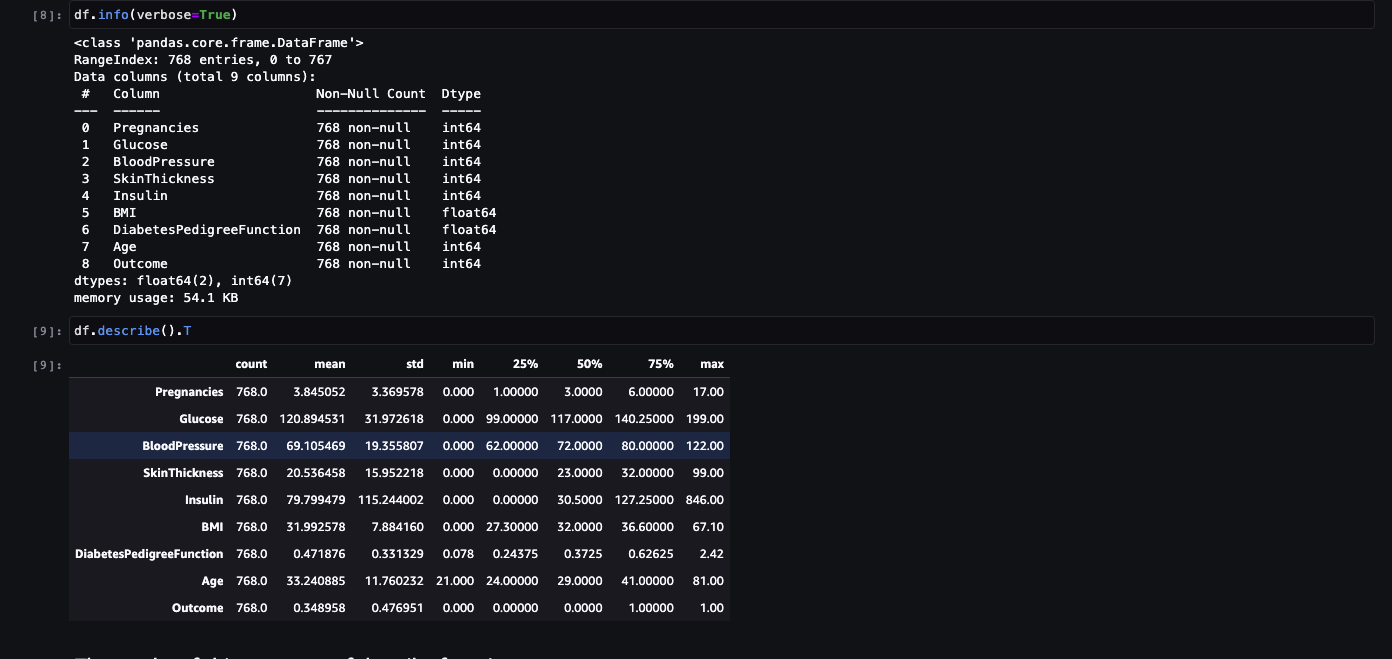
\includegraphics{describe.png}
\caption{The describe function results}
\end{figure}

\textbf{The results of this summary of describe function.} There are
some value of below listed columns have zero minimum, the value of zero
does indicates missing value. Following columns or variables have an
invalid zero value:

\begin{itemize}
\tightlist
\item
  Glucose
\item
  BloodPressure
\item
  SkinThickness
\item
  Insulin
\item
  BMI
\end{itemize}

\hypertarget{exploratory-visualization}{%
\subsection{Exploratory Visualization}\label{exploratory-visualization}}

\hypertarget{data-distribution}{%
\subsubsection{Data Distribution}\label{data-distribution}}

A left-skewed distribution has a long left tail. Left-skewed
distributions are also called negatively-skewed distributions. That's
because there is a long tail in the negative direction on the number
line. The mean is also to the left of the peak.

Figure 2 below shows data distribution.

\begin{figure}
\centering
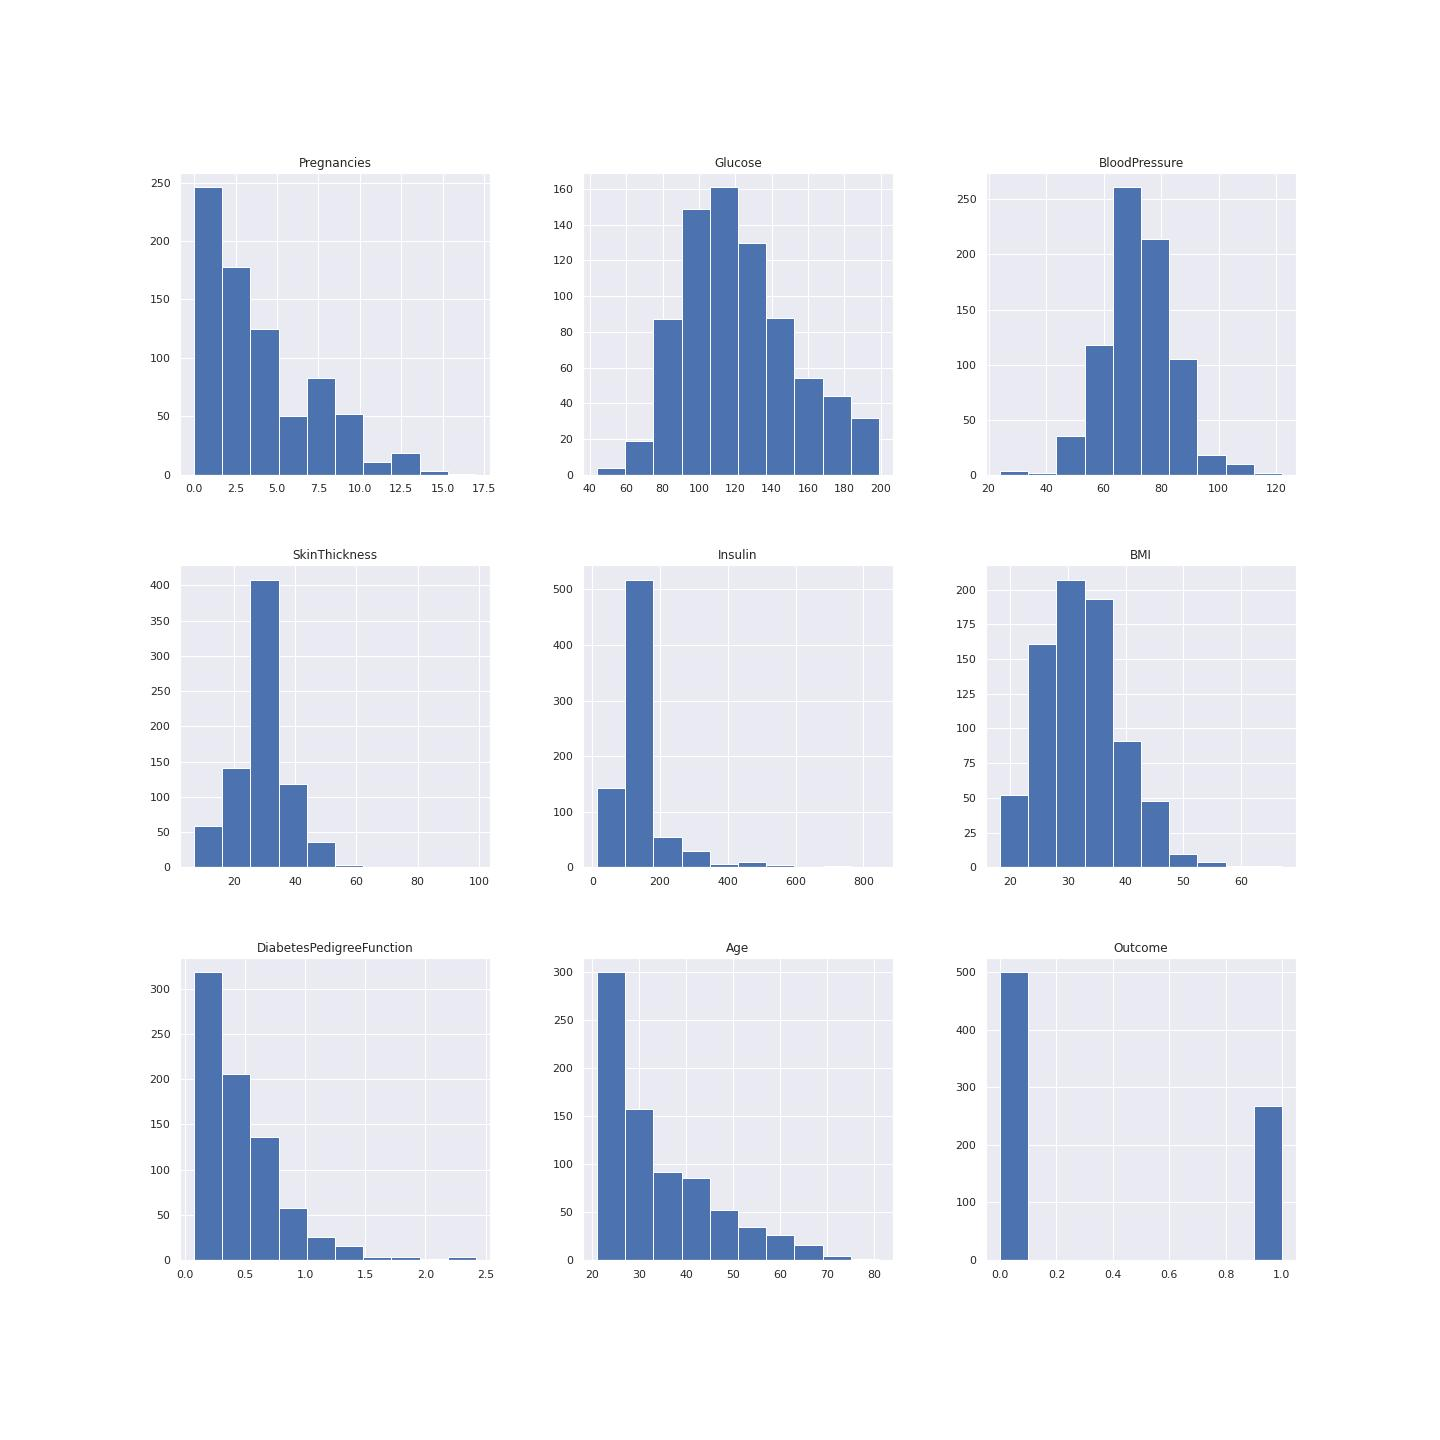
\includegraphics{clean.jpg}
\caption{Data Distribution}
\end{figure}

Aright-skewed distribution has a long right tail. Right-skewed
distributions are also called positive-skew distributions. That's
because there is a long tail in the positive direction on the number
line. The mean is also to the right of the peak.

This data is mostly left skewed for example the pregrancy plot, insulin,
age and diabetes pedigree function.

\hypertarget{correlation-visualisation}{%
\subsubsection{Correlation
visualisation}\label{correlation-visualisation}}

Heatmap is good method to visualize correlation between features. This
heatmap helps to know the following pairs had a positive correlation
coeffiecient between them as compared to other parameters.

\begin{itemize}
\tightlist
\item
  Pregnancies and age
\item
  Insulin and Skin thickness
\item
  BMI and Skin thickness
\item
  Insulin and Glucose
\end{itemize}

Glucose and BMI values are related the most. This indicates the two
parameters need special attention.

The heatmap figure 3 shows correlation coeficient

\begin{figure}
\centering
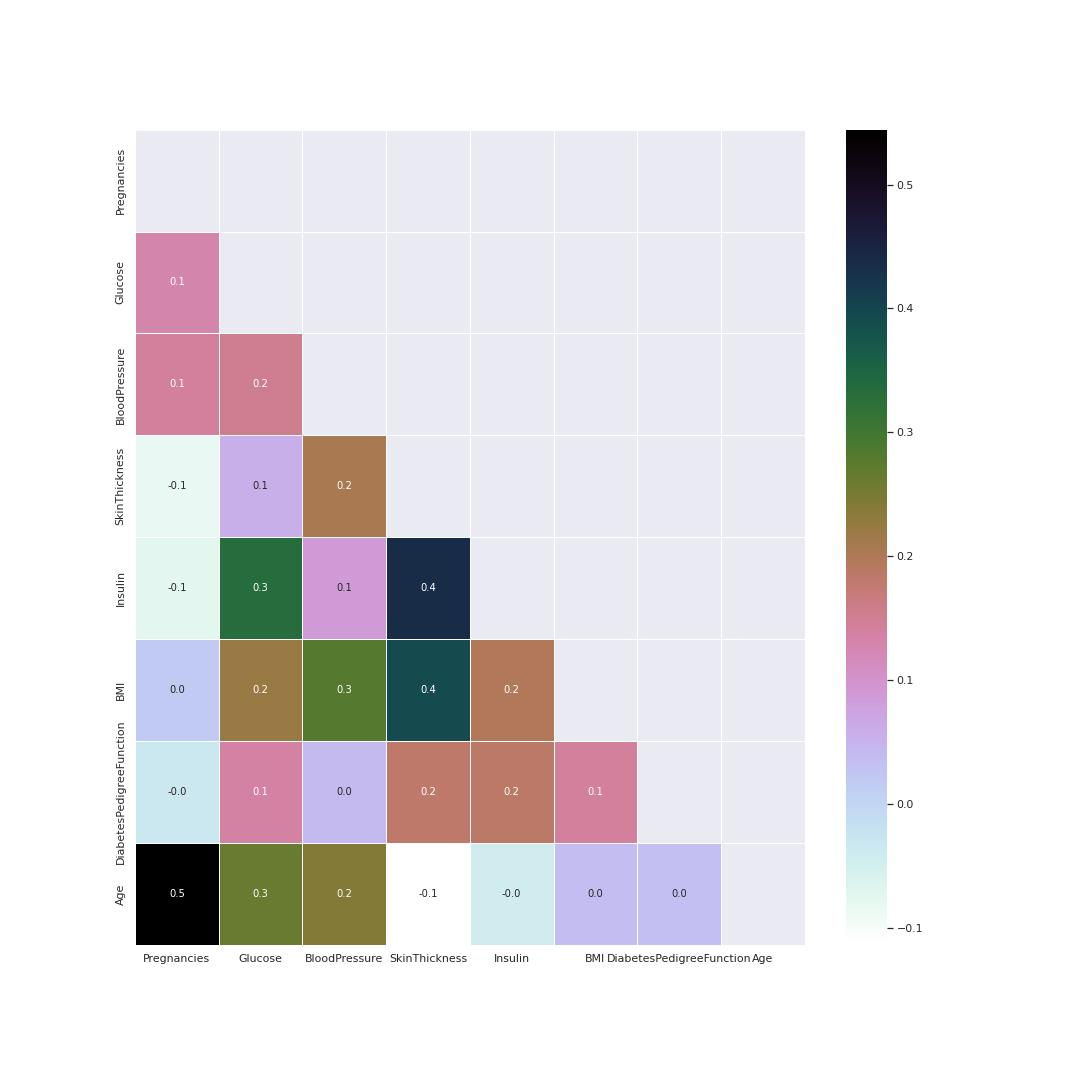
\includegraphics{Corr.jpg}
\caption{Heat map Correlation Coeffi}
\end{figure}

\hypertarget{true-diabetes-distribution}{%
\subsubsection{True Diabetes
Distribution}\label{true-diabetes-distribution}}

A violin plot is a hybrid of a box plot and a kernel density plot, which
shows peaks in the data. It is used to visualize the distribution of
numerical data. Unlike a box plot that can only show summary statistics,
violin plots depict summary statistics and the density of each
variable.\textsuperscript{\protect\hyperlink{ref-joel}{4}}

To understand data we have to plot data using violin visualization. This
plotting shows where the outcome of diabetes was 1. This shows the
distribution of the diabetes resulting from different factors. This
gives us clear picture that Glucose, BMI and Insulin had the most effect
on the outcome value. This also determines on the data division for
model training and model testing. The median age is 35 of those having
diabetes according the violin plot with the higher probability. Figure 4
shows the violin plots where the outcome is 1

\begin{figure}
\centering
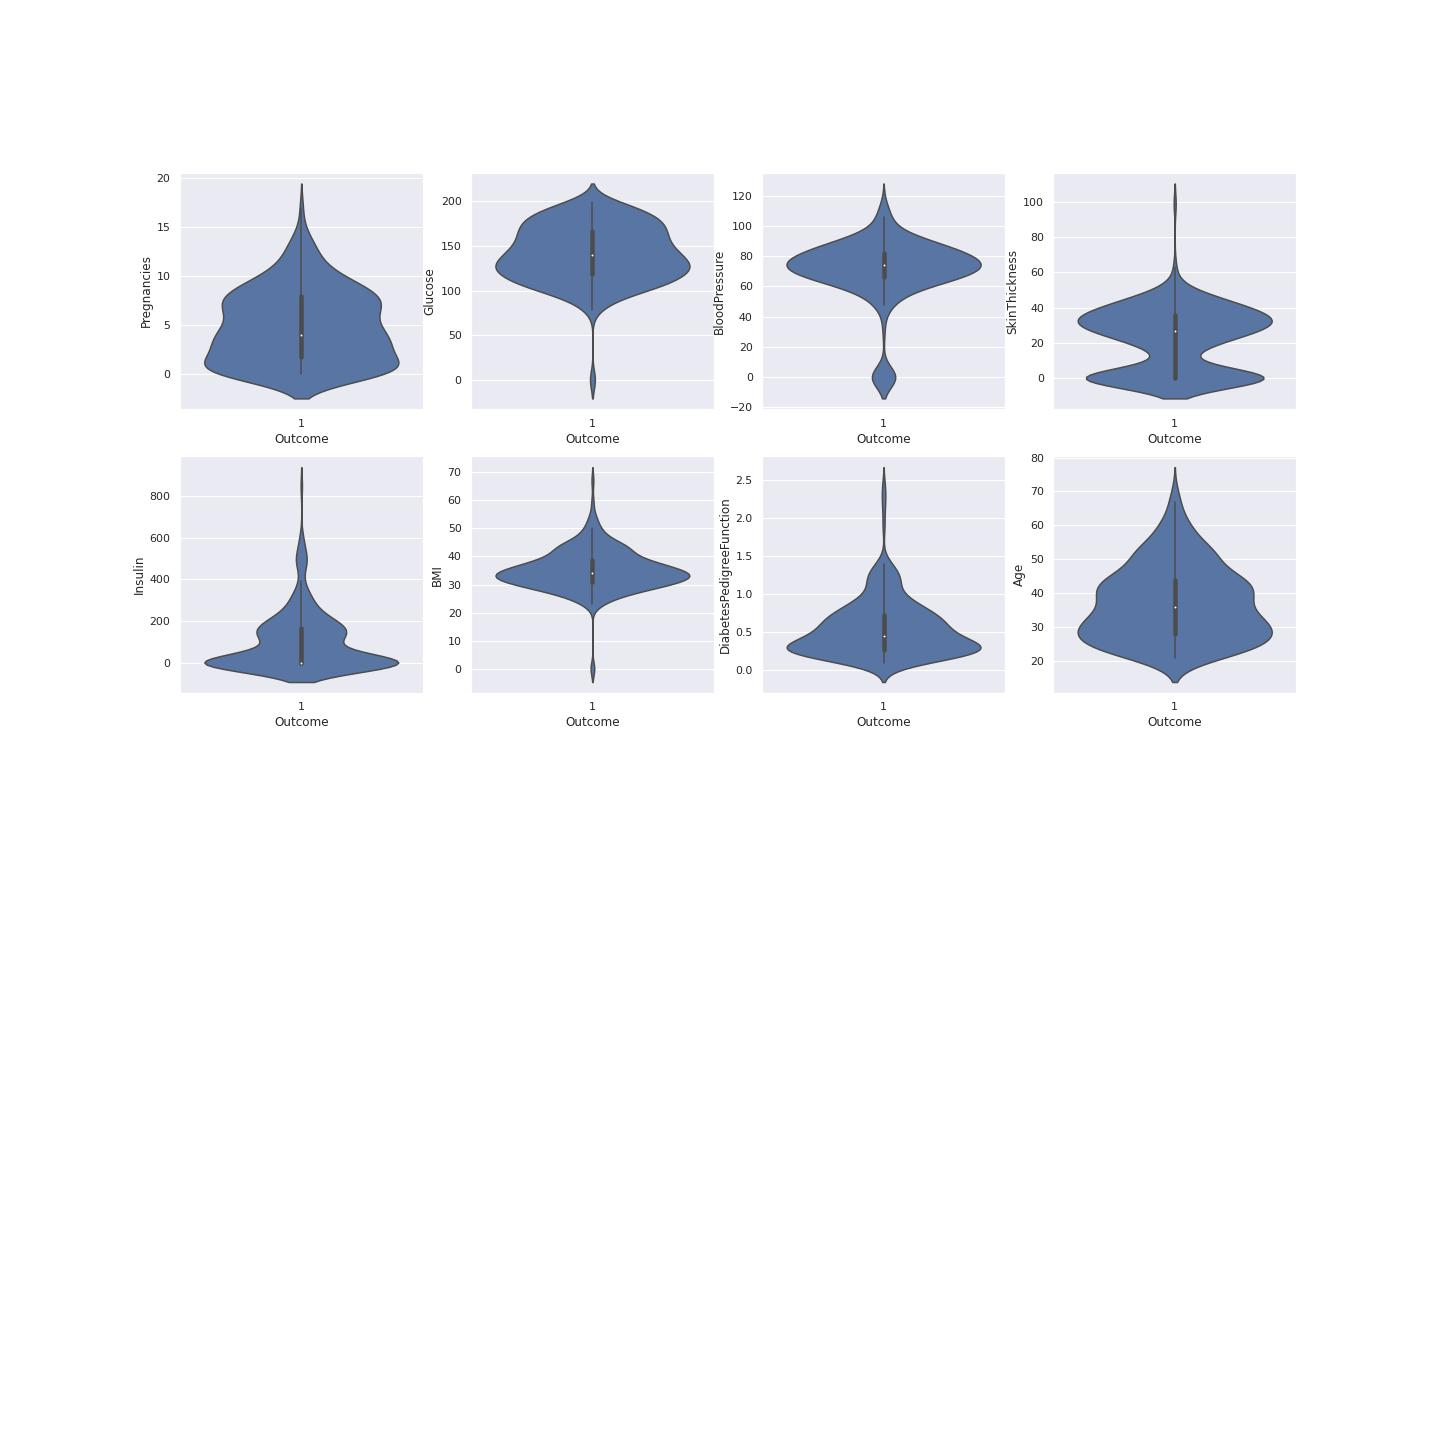
\includegraphics{truediab.jpg}
\caption{True Diabetes}
\end{figure}

\hypertarget{false-diabetes-distribution}{%
\subsubsection{False Diabetes
Distribution}\label{false-diabetes-distribution}}

To understand data we have to plot data using violin visualization. This
plotting shows where the outcome of diabetes was 0. Figure 5 shows the
violin plots where the outcome is 0

\begin{figure}
\centering
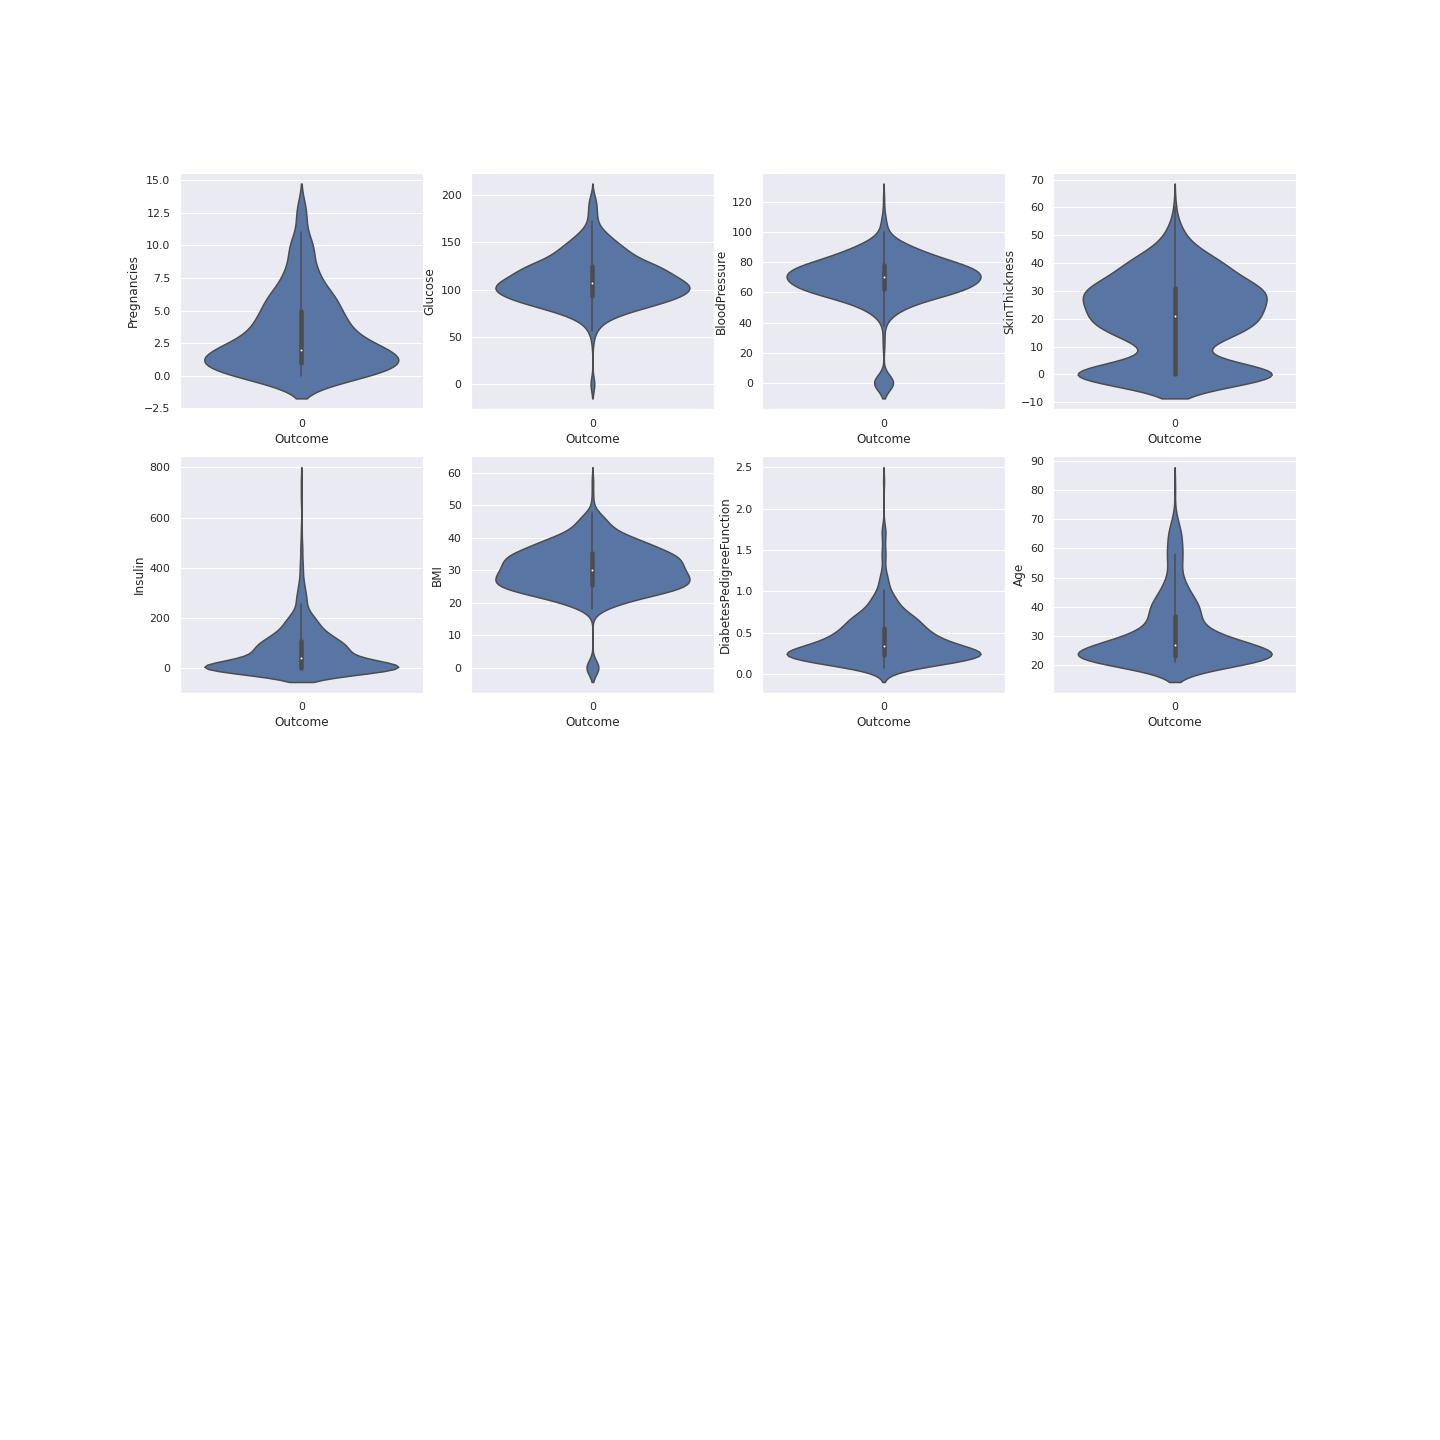
\includegraphics{falsediab.jpg}
\caption{False Diabetes}
\end{figure}

\hypertarget{algorithms-and-techniques}{%
\subsection{Algorithms and Techniques}\label{algorithms-and-techniques}}

AutoGluon automates machine learning tasks enabling you to easily
achieve strong predictive performance in your applications. With just a
few lines of code, you can train and deploy high-accuracy machine
learning and deep learning models on image, text, time series, and
tabular data.

AutoGluon enables easy-to-use and easy-to-extend AutoML with a focus on
automated stack ensembling, deep learning, and real-world applications
spanning image, text, and tabular
data.\textsuperscript{\protect\hyperlink{ref-auto}{2}}

\hypertarget{benchmark}{%
\subsection{Benchmark}\label{benchmark}}

The benchmark used was DecisionTreeClassifier algorithm

\begin{lstlisting}[language=python]
from sklearn.tree import DecisionTreeClassifier
from sklearn.model_selection import train_test_split
from sklearn import tree

X=df[df.columns[0:-1]]
Y=df[df.columns[-1]]


X_train,X_test,y_train,y_test = train_test_split(X,Y,stratify=Y,random_state=42)
clf = DecisionTreeClassifier(max_depth=4,random_state=0)
clf.fit(X_train,y_train)
print("Accuracy on training set: {:.3f}".format(clf.score(X_train,y_train)))
print("Accuracy on test set: {:.3f}".format(clf.score(X_test,y_test)))

Accuracy on training set: 0.818
Accuracy on test set: 0.766

\end{lstlisting}

\hypertarget{why-use-a-decision-tree}{%
\subsubsection{Why use a decision tree?}\label{why-use-a-decision-tree}}

\begin{itemize}
\item
  The advantages of using a decision tree are that:
\item
  They can be easy to interpret (depending on the size of your data and
  the depth of your tree)
\item
  They can handle both numeric and categorical data through scikit-learn
\item
  They can limit the influence of poor predictors in your model
\end{itemize}

\hypertarget{methodology}{%
\section{Methodology}\label{methodology}}

\hypertarget{data-preprocessing}{%
\subsection{Data Preprocessing}\label{data-preprocessing}}

Data was diveded into training set and testing set. The training set was
70 percent of the whole data while the testing set was 30 percent of the
data.

\begin{lstlisting}[language=python]
train = df.sample(frac=0.7, random_state=42)
test = df.drop(train.index)

label = "Outcome"
y_test = test[label]
X_test = test.drop(columns=[label])

\end{lstlisting}

\hypertarget{implementation}{%
\subsection{Implementation}\label{implementation}}

The platfrom for implimentation was AWS sagemaker studio. The data was
stored in AWS S3 after it was devided for training set and testing set.
The procedure for that was to create an S3 bucket using a script.

\begin{lstlisting}[language=python]

import os
import sys
import boto3
import sagemaker
from time import sleep
from collections import Counter
import numpy as np
import pandas as pd
from autogluon.tabular import TabularPredictor  
from sagemaker import get_execution_role, local, Model, utils, s3
from sagemaker.estimator import Estimator
from sagemaker.predictor import Predictor
from sagemaker.serializers import CSVSerializer
from sagemaker.deserializers import StringDeserializer
from sklearn.metrics import accuracy_score, classification_report
from IPython.core.display import display, HTML
from IPython.core.interactiveshell import InteractiveShell
import matplotlib.pyplot as plt
import seaborn as sns
sns.set()
import warnings
warnings.filterwarnings('ignore')
import missingno as msno
%matplotlib inline
session = sagemaker.Session()
bucket = session.default_bucket()
prefix = "sagemaker/autogluon-tabular"
region = session.boto_region_name
role = get_execution_role()
client = session.boto_session.client("sts", region_name=region, endpoint_url=utils.sts_regional_endpoint(region))



\end{lstlisting}

\hypertarget{training}{%
\subsubsection{Training}\label{training}}

The model was trained using AUTOML
autogluon\textsuperscript{\protect\hyperlink{ref-auto}{2}}

\begin{lstlisting}[language=python]
%%time

predictor = TabularPredictor(label='Outcome', eval_metric='roc_auc',
                             ).fit(train_data=train_s3_path,
                                  time_limit=600,
                                  presets=['best_quality',
                                  'optimize_for_deployment'],)
\end{lstlisting}

\begin{verbatim}
                    model  score_val  pred_time_val    fit_time  pred_time_val_marginal  fit_time_marginal  stack_level  can_infer  fit_order
0     WeightedEnsemble_L2   0.849699       0.947987  235.299451                0.000524           0.249235            2       True          4
1       LightGBMXT_BAG_L1   0.848956       0.128012   40.415414                0.128012          40.415414            1       True          1
2  NeuralNetFastAI_BAG_L1   0.831127       0.355836  100.760741                0.355836         100.760741            1       True          2
3   NeuralNetTorch_BAG_L1   0.830445       0.463615   93.874062                0.463615          93.874062            1       True          3

model   score_val   pred_time_val   fit_time    pred_time_val_marginal  fit_time_marginal   stack_level can_infer   fit_order
0   WeightedEnsemble_L2 0.849699    0.947987    235.299451  0.000524    0.249235    2   True    4
1   LightGBMXT_BAG_L1   0.848956    0.128012    40.415414   0.128012    40.415414   1   True    1
2   NeuralNetFastAI_BAG_L1  0.831127    0.355836    100.760741  0.355836    100.760741  1   True    2
3   NeuralNetTorch_BAG_L1   0.830445    0.463615    93.874062   0.463615    93.874062   1   True    3
\end{verbatim}

\begin{figure}
\centering
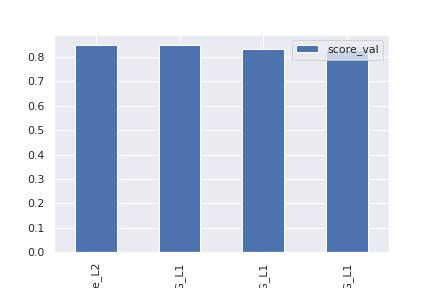
\includegraphics{leaderboard.jpg}
\caption{Leaderboard}
\end{figure}

\hypertarget{refinement}{%
\subsection{Refinement}\label{refinement}}

The refinement was to tune the hyperparameters and predict using one
model and it was done two times. The aim was to observe the performance
of prediction.

\hypertarget{fine-tuning-hyperparamters}{%
\subsubsection{Fine-tuning
hyperparamters}\label{fine-tuning-hyperparamters}}

The finetuning of the parameters set to `very\_light' as the code snipet
shows below.

\begin{lstlisting}[language=python]
%%time

predictor = TabularPredictor(label='Outcome', 
                             eval_metric='roc_auc',
                             ).fit(train_data=train_s3_path,
                                  time_limit=600,
                                  presets=['best_quality', 'optimize_for_deployment'],
                                  hyperparameters='very_light',
                                  )
\end{lstlisting}

There was not much improvement after hyperparameter tuning as the snipet
shows the model performance.

\begin{verbatim}
                     model  score_val  pred_time_val    fit_time  pred_time_val_marginal  fit_time_marginal  stack_level  can_infer  fit_order
0     WeightedEnsemble_L2   0.849699       0.947987  235.299451                0.000524           0.249235            2       True          4
1       LightGBMXT_BAG_L1   0.848956       0.128012   40.415414                0.128012          40.415414            1       True          1
2  NeuralNetFastAI_BAG_L1   0.831127       0.355836  100.760741                0.355836         100.760741            1       True          2
3   NeuralNetTorch_BAG_L1   0.830445       0.463615   93.874062                0.463615          93.874062            1       True          3

model   score_val   pred_time_val   fit_time    pred_time_val_marginal  fit_time_marginal   stack_level can_infer   fit_order
0   WeightedEnsemble_L2 0.849699    0.947987    235.299451  0.000524    0.249235    2   True    4
1   LightGBMXT_BAG_L1   0.848956    0.128012    40.415414   0.128012    40.415414   1   True    1
2   NeuralNetFastAI_BAG_L1  0.831127    0.355836    100.760741  0.355836    100.760741  1   True    2
3   NeuralNetTorch_BAG_L1   0.830445    0.463615    93.874062   0.463615    93.874062   1   True    3
\end{verbatim}

\begin{figure}
\centering
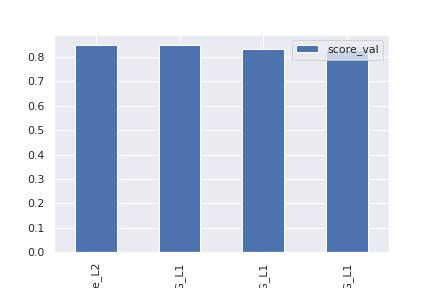
\includegraphics{leaderboard_hyper_tune.jpg}
\caption{Leaderboard after tuning hyperparameters}
\end{figure}

\hypertarget{results}{%
\section{Results}\label{results}}

The results of Autogluon training can be seen in the summary below.

\begin{verbatim}

predictor.fit_summary(show_plot=True)

*** Summary of fit() ***
Estimated performance of each model:
model  score_val  pred_time_val    fit_time  pred_time_val_marginal  fit_time_marginal  stack_level  can_infer  fit_order
0     WeightedEnsemble_L2   0.849699       0.910417  242.822065                0.000679           0.457114            2       True          4
1       LightGBMXT_BAG_L1   0.848956       0.067625   41.802209                0.067625          41.802209            1       True          1
2  NeuralNetFastAI_BAG_L1   0.831127       0.364630  104.587116                0.364630         104.587116            1       True          2
3   NeuralNetTorch_BAG_L1   0.830445       0.477483   95.975625                0.477483          95.975625            1       True          3
Number of models trained: 4
Types of models trained:
{'StackerEnsembleModel_TabularNeuralNetTorch', 'WeightedEnsembleModel', 'StackerEnsembleModel_NNFastAiTabular', 'StackerEnsembleModel_LGB'}
Bagging used: True  (with 5 folds)
Multi-layer stack-ensembling used: False 
Feature Metadata (Processed):
(raw dtype, special dtypes):
('float', []) : 2 | ['BMI', 'DiabetesPedigreeFunction']
('int', [])   : 6 | ['Pregnancies', 'Glucose', 'BloodPressure', 'SkinThickness', 'Insulin', ...]
Plot summary of models saved to file: AutogluonModels/ag-20230310_110459/SummaryOfModels.html
*** End of fit() summary ***
\end{verbatim}

\hypertarget{model-evaluation}{%
\subsection{Model Evaluation}\label{model-evaluation}}

The model was evaluated by using predctor.evaluate command which is a
built in command from the autogluon model. The result of the execution
is shown in the script below.

\begin{verbatim}
predictor.evaluate(test_s3_path)

Loaded data from: s3://sagemaker-us-east-1-495962688195/sagemaker/autogluon-tabular/data/test.csv | Columns = 9 / 9 | Rows = 230 -> 230
Evaluation: roc_auc on test data: 0.8274792522424343
Evaluations on test data:
{
    "roc_auc": 0.8274792522424343,
    "accuracy": 0.7478260869565218,
    "balanced_accuracy": 0.6872327940313522,
    "mcc": 0.41186364034362855,
    "f1": 0.5735294117647058,
    "precision": 0.6842105263157895,
    "recall": 0.4936708860759494
}
{'roc_auc': 0.8274792522424343,
 'accuracy': 0.7478260869565218,
 'balanced_accuracy': 0.6872327940313522,
 'mcc': 0.41186364034362855,
 'f1': 0.5735294117647058,
 'precision': 0.6842105263157895,
 'recall': 0.4936708860759494}
\end{verbatim}

\begin{itemize}
\item
  The roc-auc is 82 percent there is diabetes.In machine learning, we
  use ROC Curves to analyze the predictive power of a classifier: they
  provide a visual way to observe how changes in our model's
  classification thresholds affect our model's performance.
\item
  Accuracy 75 percent shows that there is diabetes
\item
  Balanced Accuracy 69 percent there is diabetes
\item
  F1 score is 0.57 showing the good performance of the model. The
  F1-score is a great way to compare the performance of multiple
  classifiers
\end{itemize}

\hypertarget{conclusion}{%
\section{Conclusion}\label{conclusion}}

AutoML frameworks offer an enticing alternative. For the novice, they
remove many of the barriers of deploying high performance ML models. For
the expert, they offer the potential of implementing best ML practices
only once (including strategies for model selection, ensembling,
hyperparameter tuning, feature engineering, data preprocessing, data
splitting, etc.), and then being able to repeatedly deploy them. This
allows experts to scale their knowledge to many problems without the
need for frequent manual intervention.

\hypertarget{reflection}{%
\subsection{Reflection}\label{reflection}}

The entire end-to-end problem solution can be summarized as the
following :

\begin{enumerate}
\def\labelenumi{\arabic{enumi}.}
\tightlist
\item
  A challenge problem and an available public dataset were found.
\item
  A suitable metric was found and implemented.
\item
  The data was downloaded and split into training, testing sets.
\item
  The data was prepared and preprocessed to be used as input for the
  classification model.
\item
  The solution model classifier was tested on unseen dataset.
\end{enumerate}

The challenging aspect of the project was the selection ECR AWS services
which was abandoned due to the lack of support

\hypertarget{improvement}{%
\subsection{Improvement}\label{improvement}}

For the improvement of our solution model, my suggestions are the
following :

\begin{enumerate}
\def\labelenumi{\arabic{enumi}.}
\tightlist
\item
  Allowing the model to have visual explainable for interplatability,
  ofcourse there is shapley values but its only for ECR(built in docker
  containers AWS). I say this since I tried to use ECR services and
  failed.
\item
  Another possible improvement is collecting a larger dataset of
  landmarks, training the model on a larger amount data, but yeah again
  it is challenging to EHR data. \newpage
\end{enumerate}

\hypertarget{references}{%
\section*{References}\label{references}}
\addcontentsline{toc}{section}{References}

\hypertarget{refs}{}
\begin{CSLReferences}{0}{0}
\leavevmode\vadjust pre{\hypertarget{ref-ehr}{}}%
\CSLLeftMargin{1. }%
\CSLRightInline{Aamna.
\href{https://kaggle.com/competitions/hw1-machine-learning-for-ehr}{HW1
machine learning for EHR}. (2023).}

\leavevmode\vadjust pre{\hypertarget{ref-auto}{}}%
\CSLLeftMargin{2. }%
\CSLRightInline{Autogluon.
\href{https://auto.gluon.ai/stable/index.html\%20(Accessed:\%2013\%20March\%202023).}{AutoML
for text, image, time series, and tabular data --- AutoGluon
documentation 0.7.0 documentation (2023).}}

\leavevmode\vadjust pre{\hypertarget{ref-volo}{}}%
\CSLLeftMargin{3. }%
\CSLRightInline{Volodkevich, A.
\href{\%20https://towardsdatascience.com/auc-and-its-implementation-in-catboost-6bc740c01f98\%20(Accessed:\%20March\%2013,\%202023)}{AUC
and its implementation in CatBoost, medium. Towards data science.}}

\leavevmode\vadjust pre{\hypertarget{ref-joel}{}}%
\CSLLeftMargin{4. }%
\CSLRightInline{Carron, J.
\href{https://mode.com/blog/violin-plot-examples/\%20(Accessed:\%20March\%2013,\%202023)}{Violin
plots 101: Visualizing distribution and probability density}.}

\end{CSLReferences}

\end{document}
